\documentclass[12pt]{article}
\usepackage{scrtime} % for \thistime (this package MUST be listed first!)
\usepackage[margin=1in]{geometry}
\usepackage{subfig}

%% Language and font encodings
\usepackage[english]{babel}
\usepackage[utf8x]{inputenc}
\usepackage[T1]{fontenc}


%% Useful packages
\usepackage{amsmath}
\usepackage{amsthm} % for theorems and proofs
\usepackage{amsfonts} % mathbb
\usepackage{graphicx}
\usepackage[colorinlistoftodos]{todonotes}
\definecolor{aqua}{RGB}{0, 128, 225}
\usepackage[colorlinks=true,citecolor=aqua,linkcolor=aqua,urlcolor=aqua]{hyperref}
\usepackage[nameinlink]{cleveref}
\usepackage{lineno}

\usepackage{fancyhdr,lastpage}
\pagestyle{fancy}
\fancyhf{} % clear all header and footer parameters
%%%\lhead{Student Name: \theblank{4cm}}
%%%\chead{}
%%%\rhead{Student Number: \theblank{3cm}}
%%%\lfoot{\small\bfseries\ifnum\thepage<\pageref{LastPage}{CONTINUED\\on next page}\else{LAST PAGE}\fi}
\lfoot{}
\cfoot{{\small\bfseries Page \thepage\ of \pageref{LastPage}}}
\rfoot{}
\renewcommand\headrulewidth{0pt} % Removes funny header line

\newcommand{\R}{{\cal R}}

\usepackage{xspace}
\newcommand{\Rlogo}{\protect
\includegraphics[height=2ex,keepaspectratio]{Rlogo.pdf}\xspace}

\title{Synchrony and Persistence of Recurrent Epidemics}
\author{ \underline{\emph{Group Name}}: \texttt{{\color{blue}The Infective Collective}}\\
\\}
\date{\today\ @ \thistime}

\begin{document}
\vfill
\maketitle 
\noindent

\underline{\emph{Group Members}}:
\begin{itemize}
{\color{blue}
\item Aurora Basinski-Ferris (basinsa@mcmaster.ca), 
\item Michael Chong (chongmy@mcmaster.ca), 
\item Sang Woo Park (parksw3@mcmaster.ca), 
\item Daniel Presta (prestad@mcmaster.ca)}
\end{itemize}
\noindent 
Date compiled: \today\ @ \thistime 

\noindent
Word Count: 

\vfill
\newpage 
\linenumbers

\section*{Executive summary}
Major North American urban centres are distributed sparsely and are loosely connected to each other through travel. This spatial structure presents challenges in the eradication of diseases and control of epidemics. Even if the disease is eradicated in one city, it may be reintroduced if infected individuals from other populations visit and interact with susceptible individuals. This phenomenon, where an eradicated disease is reintroduced via contact with another city, is called “the rescue effect”.

The rescue effect, in theory, can be avoided if eradication of the disease happens simultaneously across all of the connected populations. Therefore, it is beneficial from a disease control perspective to have “synchronous” or “coherent” patterns of prevalence between the populations. That is, to have temporal peaks and troughs in prevalence occurring at the same time in every city. In this way, cities that have eradicated the disease are at lower risk of reintroduction since other populations would also experience low incidence of the disease. Via coordinated vaccination, we may be able to achieve this simultaneous and thus sustainable eradication of the disease.

In this study, we have examined a mathematical disease model with two subpopulations to investigate the conditions that result in coherence between cities. We have found that coherence is more likely to occur between cities whose infected residents spend more time interacting with the residents of the other city. For cities where infected residents spend only a small amount of time interacting with residents in the other city, we find that coherence in prevalence patterns is more likely for diseases which are more infectious. 

Based on these preliminary findings, we can make some initial suggestions regarding disease control strategies. The primary implication from this study is that cities which are well connected likely have synchronous patterns of prevalence. Therefore, they may benefit from coordinated vaccination and quarantine strategies that simultaneously eradicate the disease and prevent the rescue effect. We also suggest that for diseases which are highly infectious, cities which appear to be only loosely connected, may still benefit from coordinated vaccination. As populations which are not part of this coordinated vaccination strategy may still have the potential to reintroduce the disease in a city, we suggest that screening is done for travel between cities that are not part of coordinated disease control efforts.

We note that the scope of this study is limited, and we made various simplifying assumptions about our disease model. First, we assumed that the contact rate among individuals throughout the year was high during school terms but low otherwise. Our results are therefore pertinent to diseases that affect children and youth, but may not generalize to diseases primarily affecting adults whose contact patterns are different. Our model also only considered two equally-sized cities whose individuals are equally likely to travel to the opposite city. Further investigation is needed to investigate whether these findings generalize to many-city systems, and to cities where there is a disparity in the population size of the cities and/or if residents of city A are more likely to travel to city B than vice versa. Although a deeper investigation of synchrony in more complicated systems is needed, this study provides some insight into the factors that affect synchrony, and suggests that coordinated vaccination may help eradicate diseases on a large scale.
\newpage

\begin{abstract}
Asynchronous epidemic dynamics across geographical regions is undesirable because it allows for diseases to be reintroduced to subpopulations where the disease has already been eradicated. Alternatively, synchrony can lead to the simultaneous extinction of the disease in all subpopulations.
In this paper, we explore synchrony and coherence between subpopulations using a two-patch discrete-time SIR model.
We find that coherence in disease dynamics is more likely to occur between highly connected populations, and that it is dependent on the basic reproductive number. 
Furthermore, we observe that the rescue effect leads to greater persistence in weakly-connected systems that incorporate demographic stochasticity.  
\end{abstract}

\tableofcontents

\section{Background}
 
Synchrony is defined as the coincident changes of time-varying characteristics (such as the prevalence of a disease) in geographically separate populations \cite{liebhold2004spatial}. Coherence is the strongest form of synchrony, in which population densities in each city or geographical patch are equal for all time \cite{earn2006global}. A coherent epidemiological system is one in which the prevalence of disease in every subpopulation becomes and remains identical.

Past work by Earn \textit{et al.} shows that spatial coherence can increase the chance of extinction in a population growth model \cite{Earn2000conservation}. 
Depending on the context and purpose, there are cases in which the relationship between synchrony and risk of extinction might be undesirable.
For example, conservation ecologists wish to prevent against coherence in animal population models to avoid all subpopulations from becoming extinct at the same time \cite{Earn2000conservation}. However, in epidemiology, extinction of pathogens is advantageous. Thus, from a public health perspective, it is useful to determine the conditions under which coherence occurs as this may aid in the eradication of disease \cite{earn1998persistence}. 

Asynchrony allows for greater persistence, as through migration of infected individuals, it enables the ``rescue effect'', and thus prevents eradication \cite{brown1977turnover}. 
The rescue effect is defined as the rebirth of a subpopulation by dispersion of individuals from neighbouring surviving subpopulations \cite{nicholson1935balance,levins1969some,adler1993migration}. 
From an epidemiological standpoint, rescue effects enable a disease that has become locally extinct (i.e. extinct in one subpopulation) to be potentially revived by dispersed infected individuals from a neighbouring subpopulation (in which an epidemic still exists).

In this paper, we attempt to examine the connection between synchrony and persistence in recurrent epidemics by using a simple epidemiological model that accounts for mixing between two subpopulations.
Here, we examine the effects of dispersal rates and changes in parameter space on synchrony and try to quantify probability of coherence and extinction using numerical simulations.

\section{Methods} \label{sec:methods}
\subsection{The model} \label{ss:deter_model}
We use a discrete time SIR (Susceptible-Infected-Recovered) model with time-dependent transmission rate and with two subpopulations (or spatial patches), based on a compartmental ODE SIR model. While individuals do not migrate between the subpopulations, we assume that a proportion $(1-m)$ of infected individuals only contact susceptible individuals in their own subpopulation, while the remaining proportion $m$ of infected individuals from each patch contact only susceptibles from the opposite subpopulation. Alternatively, we can interpret $m$ as the mean proportion of time that an infected individual spends in the opposite patch. Since an equal proportion $m$ of infectives from each patch contact susceptibles from the opposite patch, we refer to this as an equal coupling connectivity structure. 

The number of individuals leaving each compartment is given by a transition probability derived from a hazard analysis (see the Supplementary Information (part?) for the full construction of the model). Let $S_k(t)$, $I_k(t)$, and $R_k(t)$ denote the number of susceptible, infected, and recovered individuals respectively in subpopulation $k$ at time $t$. Then our model is given by 
\begin{equation}
\label{eq:discretedeterministic}
\begin{aligned}
S_{k}(t+\Delta t) &= \nu_k(t) + S_k(t) - S_{k, \tiny{\textrm{leave}}}(t)\\
I_{k}(t+\Delta t) &= i_k(t) + I_k(t) - I_{k, \tiny{\textrm{leave}}}(t)\\
R_{k}(t+\Delta t) &= r_k(t) + R_k(t) - R_{k, \tiny{\textrm{leave}}}(t)
\end{aligned}
\end{equation}
where 
\begin{equation} \label{eq:SIR-det}
\begin{aligned}
S_{k, {\tiny\textrm{leave}}}(t) &= \left(1 - \exp \left(-\left(\sum_{j=1}^n \beta(t) m_{ij} I_j(s) + \mu \right) \Delta t \right) \right) S_i(t)\\
I_{i, \tiny{\textrm{leave}}}(t) &= (1 - \exp(-(\gamma + \mu)\Delta t)) I_i(t) \\
R_{i, \tiny{\textrm{leave}}}(t) &= (1 - \exp(-\mu \Delta t)) R_i(t) \\
i_k(t) &= \frac{\sum_{j=1}^n \beta(t) m_{kj} I_j(s)}{\sum_{j=1}^n \beta(t) m_{kj} I_j(s) + \mu} S_{k, \tiny{\textrm{leave}}}(t)\\
r_k(t) &= \frac{\gamma}{\gamma + \mu} R_{k, \tiny{\textrm{leave}}}(t)\\
\nu_k(t) &= S_{k, \tiny{\textrm{leave}}}(t) - i_k(t) + I_{k, \tiny{\textrm{leave}}}(t) - r_k(t).
\end{aligned}
\end{equation}
Here, $\beta(t)$ is the transmission rate, $m_{k,j}$ is the proportion of infected individuals in patch $j$ who interact with susceptibles in patch $k$, $\gamma$ is the per capita recovery rate, and $\mu$ is the per capita natural death rate. The birth rate $\nu_k(t)$ is defined such that the population size remains constant at $N = 1,000, 000$ individuals in each patch. Unless otherwise stated, we choose parameters that reflect measles-like dynamics. In particular, $\gamma = 365/13 \textrm{ years}^{-1}$ (reflecting the sum of an 8 day exposed period and 5 day infectious period). We take $\Delta t = 1/365$ years, $\gamma = 0.02 \textrm{ years}^{-1}$.
Since transmission rates for childhood diseases depend on the contact rates between children \cite{keeling2002understanding}, we used a step-function as our time-dependent transmission rate. We defined $\beta (t)$ similar to \cite{bauch2003interepidemic} where the transmission rate is high during the school term and low otherwise (see Supplementary Information for details):
\begin{equation}
\begin{aligned}
\beta (t) &=
\begin{cases} b_0 (1 + 2(1 - p_s) b_1) &\mbox{school days} \\
b_0 (1 - 2 p_s b_1) & \mbox{non-school days}
\end{cases},
\end{aligned}
\end{equation}
where $b_0$ is the mean transmission rate, $b_1 = 0.25$ is the amplitude of term-time forcing, and $p_s = 0.7589$ is the approximate proportion of the year that falls in the school term. We define $b_0$ based on the $\R_0$ value of the simulation, where $\R_0 = b_0 N / (\gamma + \mu) \approx b_0 N / \gamma$.

The single-patch dynamics of this model are similar to that of a more conventional ODE SIR model (for instance, the SIR model given by \cite{earn2000simple}). The bifurcation diagram shown in \Cref{fig:bifurcation} summarizes the single-patch dynamics for this model.

\begin{figure}
\centering
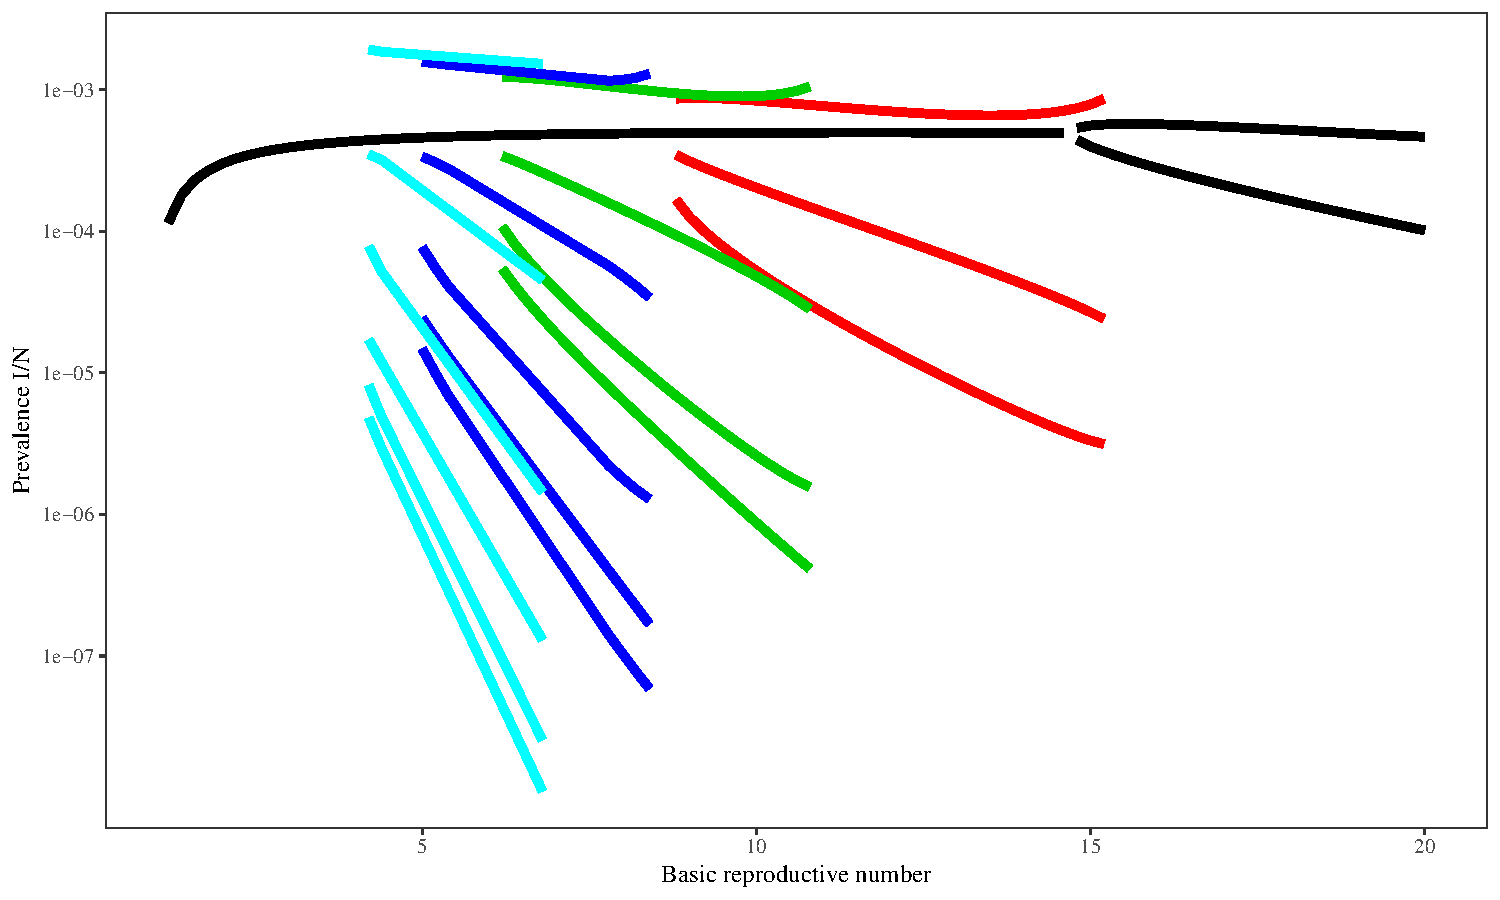
\includegraphics[width=\textwidth]{supplementary/bifurcation.pdf}
\caption{\textbf{The bifurcation diagram for a single patch term-time forced discrete time SIR model.}
The bifurcation diagram shows incidence on January 1 as a function of the basic reproductive number $\R_0$. The fixed parameter values are $\gamma = 365/13 \textrm{ years}^{-1}$, $\Delta t = 1/365$ years, $\gamma = 0.02 \textrm{ years}^{-1}$. The term-time forcing $\beta(t)$ corresponds to school terms in Toronto. See \Cref{ss:deter_model} for explanations of these parameters. For sufficiently high $\R_0$, we observe only a biannual cycle. As $\R_0$ decreases, 3-, 4-, 5-, and 6-year cycles can occur. For sufficiently small $\R_0$, only a single annual cycle can occur. }
\label{fig:bifurcation}
\end{figure}

\subsection{Stochasticity} \label{ss:stoch_model}
This discrete time model arising from a probabilistic argument allows for a natural implementation of demographic stochasticity. We add stochasticity to this model by treating the number of individuals that transition between compartments as a binomial random variable defined using the transition probabilities in the base model. That is, we replace the terms in \Cref{eq:SIR-det} with
\begin{equation}
\label{eq:stochastic}
\begin{aligned}
S_{k, \tiny{\textrm{leave}}}(t) &= \mathrm{Binom}\left(S_k(t), 1 - \exp \left(-\left(\sum_{j=1}^n \beta(t) m_{ij} I_j(s) + \mu \right) \Delta t \right)\right)\\
I_{k, \tiny{\textrm{leave}}}(t) &= \mathrm{Binom}\left(I_k(t), 1 - \exp \left(-\left(\gamma + \mu \right) \Delta t \right)\right)\\
R_{k, \tiny{\textrm{leave}}}(t) &= \mathrm{Binom}\left(R_k(t), 1 - \exp \left(-\mu \Delta t \right)\right)\\
i_k(t) &= \mathrm{Binom}\left(S_{k, \tiny{\textrm{leave}}}(t), \frac{\sum_{j=1}^n \beta(t) m_{ij} I_j(s)}{\sum_{j=1}^n \beta(t) m_{ij} I_j(s) + \mu}\right)\\
r_k(t) &= \mathrm{Binom}\left(R_{k, \tiny{\textrm{leave}}}(t), \frac{\gamma}{\gamma + \mu}\right) \\
b_k(t) &= S_{k, \tiny{\textrm{leave}}}(t) - i_k(t) + I_{k, \tiny{\textrm{leave}}}(t) - r_k(t).
\end{aligned}
\end{equation}

\subsection{Implementation}
The model was implemented using the \texttt{Rcpp} package for the \Rlogo programming language. The source code is available in the Supplementary Information, as well as online at \url{https://github.com/The-Infective-Collective/math4mb3}.  

\subsection{Measurement of coherence}
\label{ss:measurement}
Below we describe a measurement of incoherence that we use to evaluate synchrony in our simulations. 
Let $\vec{I} (t) = (I_1(t), \dots, I_n(t))$ denote the number of individuals infected at time $t$ in patches $k = 1, \dots, n$. We then define incoherence $\delta$ at time $t$ as
$$
\delta(t) = || \vec{I}(t) - \langle \vec{I} (t) \rangle \vec{e}||_2,
$$
where $\langle \vec{I} (t) \rangle = \sum_{k=1}^n I_k(t) / n$ denotes the mean prevalence among the patches at time $t$, and $\vec{e} = (1, \dots, 1)$. We therefore say the system is coherent when $\delta$ is small to within $0 \leq \delta < 100$. 

\section{Results} \label{sec:numerical}
\subsection{Deterministic model} \label{ss:deterministic}
In the deterministic case, we are most interested in investigating the dependency of coherence on the parameter space. To aid in our investigations of coherence, we generate an approximate probability of coherence by performing runs with 100 different initial conditions at set parameters, and observing if the average coherence (by the metric given in \Cref{sec:methods}) is above or below an absolute threshold (yielding an assignment of `incoherent’ and `coherent’, respectively). Our results show that this probability of coherence has a dependency on $\R_0$ at low mixing proportions. An example of this is shown in \autoref{fig:deterministic_panel}, where with a mixing proportion of $0.1\%$ ($m = 0.001$), we see a large variation in the probability of coherence across the parameter space. In particular, we note that the probability of coherence behaviour may have some interplay with the single patch dynamics (given by the bifurcation diagram). We tend to see that large changes in the probability of coherence coincides with the beginning of cycles in a single patch. For example, the increase in probability of coherence around $\R_0=4$ coincides with the beginning of the 6-cycle shown in cyan, while the large decrease around $\R_0=8$ coincides with the beginning of the 3-cycle shown in red. 

The probability of coherence also has a dependency on the mixing proportion between the two patches. For example, with a mixing proportion of $0.01\%$ ($m = 0.0001$), we see that the probability of coherence is lower than the probabilities at $0.1\%$ for almost all $\R_0$ values (see \autoref{fig:deterministic_panel}). In fact, we note that the probability of coherence is less than 1 for all $\R_0$ values greater than 1. Similarly, the mean probability of coherence for $0.1\%$ ($m=0.001$) mixing is around $0.689$, while for $0.01\%$ ($m=0.0001$) it is $0.459$. We similarly see that with higher mixing proportions, the probability of coherence is higher. A similar investigation with a mixing proportion of $1\%$ ($m=0.01$) shows that the probability of coherence is, on average, higher than the previous two investigations (see \autoref{fig:deterministic_panel}). In fact, the probability of coherence is $1$ across the parameter space except for a small region between $\R_0=2.2$ and $\R_0=3.0$ (inclusive). The mean probability of coherence for $1\%$ ($m=0.01$) mixing is 0.997. This trend continues as we increase the mixing proportion further. When we investigate $10\%$ ($m=0.1$) mixing and $50\%$ ($m=0.5$) mixing, we note that across the whole $\R_0$ parameter space, all of our 100 runs demonstrate coherence (see \autoref{fig:deterministic_panel}).

\begin{figure}
\centering
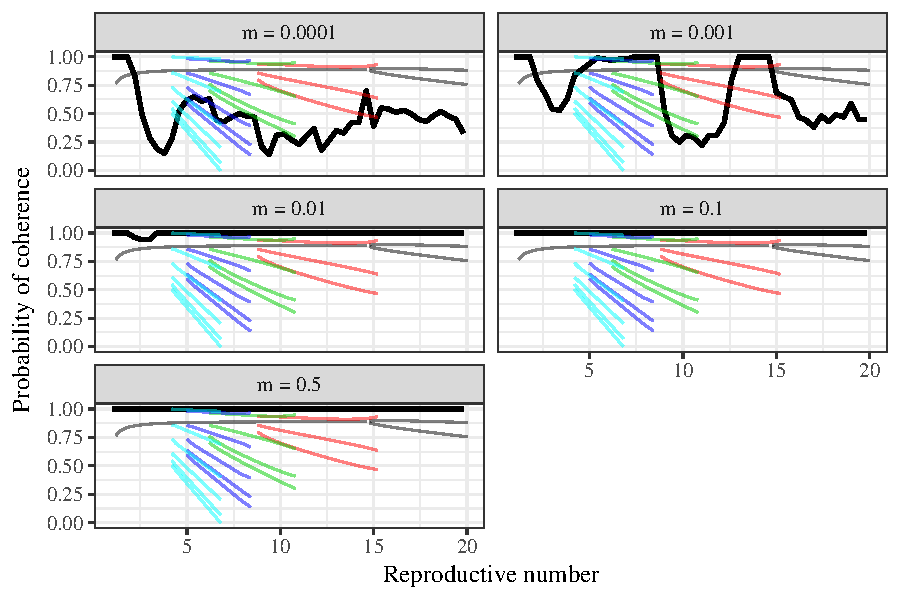
\includegraphics[width=\textwidth]{supplementary/probabilitycoherence}
\caption{\textbf{Probability of coherence in deterministic simulations.} The probability of coherence for various mixing proportions is shown in each part of this Figure. In each subfigure, the probability of coherence at a given mixing proportion is shown as the thick black line which overlays the bifurcation diagram for a single patch. The probability of coherence is generated by performing 100 runs (all starting with random initial conditions) for 100 years. Then, we check the proportion of these runs that show coherence when averaging the last 2 years - a run is deemed coherent if the coherence measure described in \Cref{ss:measurement} is below an absolute threshold of 100. Moving across rows from left to right (and then from the first row to the last row), the mixing proportions shown are $0.01\%$, $0.1\%$, $1\%$, $10\%$, and $50\%$.}
\label{fig:deterministic_panel}
\end{figure}
\subsection{Stochastic model} \label{ss:stochastic}

We observe that when stochasticity is added, coherence becomes difficult to define, since the random variance at each time step enables a potential change in the degree of synchrony within a trajectory. The change from synchronous behavior to asynchronous behavior is displayed in \autoref{fig:stoch1_shift}.

\begin{figure}[h]
    \centering
    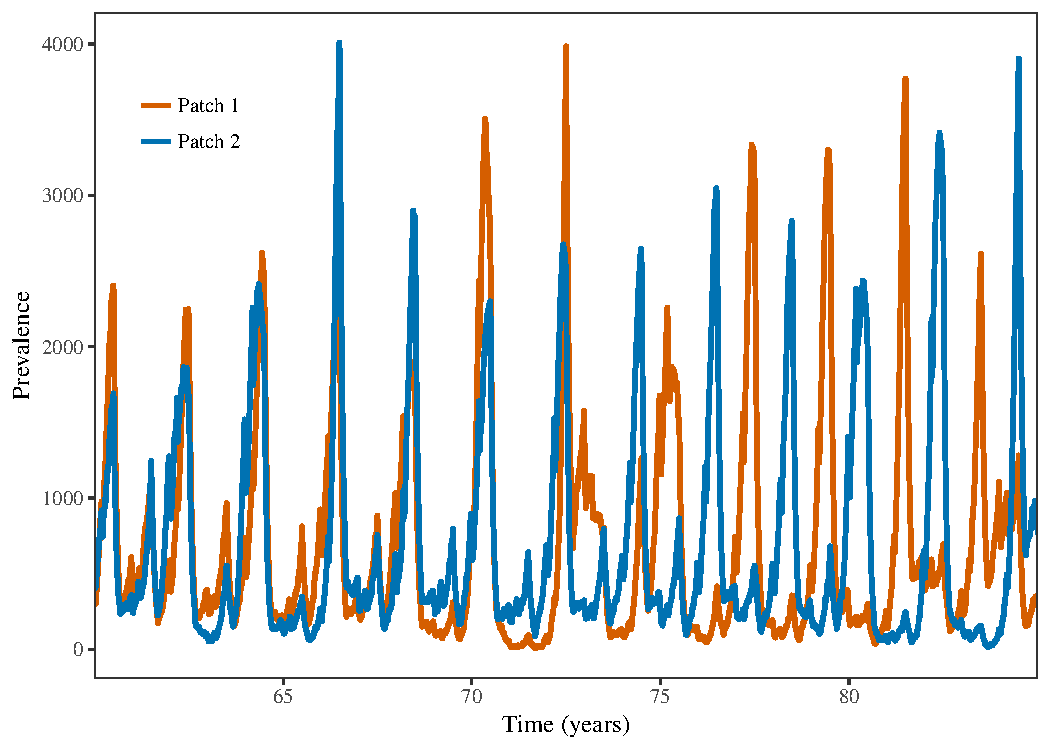
\includegraphics[width=\textwidth]{supplementary/stochastic_illustrate.pdf}
    \caption{\textbf{Observed synchronous and asynchronous behavior in a two patch, stochastic model.} Note that the trajectory displays synchronous behavior at first, before developing into to an asynchronous system after roughly 12.5 years. A mixing proportion of 0.1\% ($m = 0.001$) was used, along with $\R_0 = 17$. In addition, we assumed that the initial conditions are given by the endemic equilibrium. The trajectory displays results from year 60 of the simulation to year 85.}
    \label{fig:stoch1_shift}
\end{figure}

In order to better understand the effects of mixing between populations in a stochastic environment, we instead analyze global and local extinction probabilities. 
We find that the sharp increases and decreases in global and local extinction probabilities coincide with the beginning of new cycles (or the end of old cycles) in the bifurcation diagram, displayed in \autoref{fig:stoch}. 
This is similar to our analysis of the deterministic model, in which sharp increases and decreases in probability of coherence are observed at cycle endpoints.

In \autoref{fig:stoch}, we observe that when the mixing proportion is as low as 0.1\% ($m = 0.001$), there is large disagreement between local extinction probability and global extinction probability, even though the shapes of the probability curves are very similar. 
When $\R_0$ is between 12.5 and 18 (the biologically relevant range for measles \cite{anderson1982directly}), local extinction probability ranges from 23\% to 65\%, while global extinction probability ranges from 0\% to 13\%. 
Near $\R_0 \approx 5$, global extinction probability is low despite the existence of a 6-cycle that have prevalence of infection as low as $10^{-8}$.

\begin{figure}[h]
    \centering
    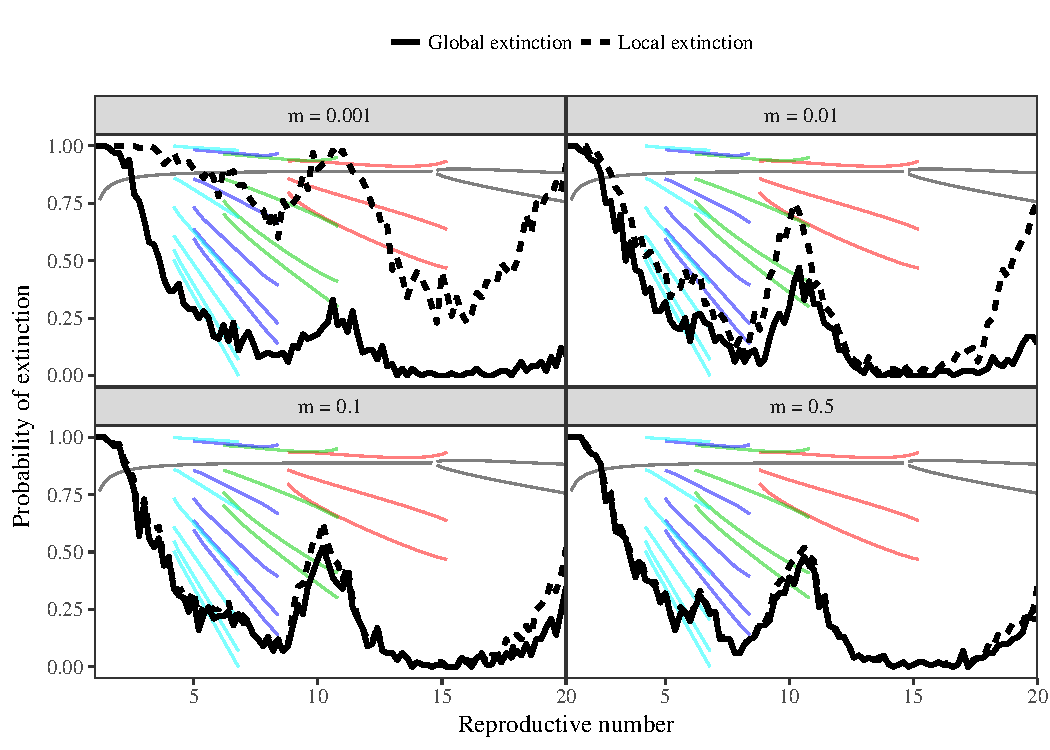
\includegraphics[width=\textwidth]{supplementary/stochastic.pdf}
    \caption{
    \textbf{Local and global extinction probabilities in stochastic simulations.}
    For each simulation, binary statistic is computed on the basis of whether local/global extinction occurred (1) or not (0). Probability of extinction is computed by proportion of 100 simulations that exhibited local/global extinctions.
    Probability of global extinction (solid line) and probability of local extinction (ashed line) are overlaid on top of the bifurcation diagram.
    }
    \label{fig:stoch}
\end{figure}

The difference in local and global extinction probabilities can be explained by the rescue effect. 
When the disease becomes locally extinct in one population, infected individuals who have dispersed from a neighboring patch to the locally extinct population can restart the epidemic, thus allowing the disease to persist longer. 
Hence, asynchrony between populations can prevent the eradication of a disease.

When there is a small amount of mixing between populations, the probability that two populations will become coherent is relatively low (\autoref{fig:deterministic_panel}).
When demographic stochasticity is introduced, attaining synchrony between the two populations is even less likely. 
However, as we increase the mixing proportion from $1\%$ to $50\%$ ($m=0.01$ to $m=0.5$), differences between local and global extinction probabilities become smaller (\autoref{fig:stoch}).
Since the prevalence of disease in two populations becomes more coherent as the mixing rate increases, the two populations are thus more likely to reach a trough in their prevalence and become extinct at a similar time. 
As would be expected from the probability of coherence results observed in the deterministic case, we find that an increase in mixing between populations leads to an increase in overall global extinction probability. When mixing proportion is 0.1\% ($m = 0.001$), global extinction probability is always less than 35\% for $\R_0 > 10$, but for all other observed $m$ values, global extinction probabilities reach approximately 50\%. 
Similar to the deterministic case, we observe that changes in the behaviour of extinction probabilities in the stochastic model are dependent on the parameter space and mixing proportion.

\section{Discussion}
\label{sec:discussion}

Understanding the persistence of an epidemic is crucial in devising effective control strategies.
Mathematical models have been successfully applied in understanding recurrent epidemics but many studies have neglected spatial structure \cite{earn2000simple, dalziel2016persistent}.
Here, we analyzed a discrete-time SIR model in two connected populations to explore the effects of mixing among population on recurrent epidemics and their synchronization.

Our key findings are (1) basic reproductive number and mixing proportion and mixing proportion play important roles in determining synchrony among populations and (2) asynchrony and synchrony have opposite effects on the persistence of an epidemic.
The dependency of the probability of coherence on both $\R_0$ and the mixing proportion may provide some insight into differences in coherence with different diseases. 
For example, \cite{rohani1999opposite} showed that introduction of vaccination in the UK for measles and whooping cough resulted in opposing changes in coherence for each disease. 
Vaccination synchronized whooping cough epidemics across UK cities while vaccination desynchronized measles epidemics. 
As the introduction of vaccination corresponds to a decrease in $\R_0$, the changes in coherence could be due to a change in coherence probability, which tends to vary with the value of the basic reproductive number. 

It is interesting that there are opposite changes in coherence even though measles and whooping cough have similar $\R_0$ values. 
Although further investigation is needed, this phenomenon could possibly be explained by differences in the mixing proportion. 
As the mixing proportion denotes the proportion of infected individuals travelling to the other patch, we could expect more debilitating diseases to have a lower mixing proportion, since infected individuals would be less likely to travel. Thus, even though measles and whooping cough share the same population, there could be mixing rate differences, since whooping cough is most infectious when it has mild symptoms similar to those of the common cold. On the other hand, the first symptoms of measles tend to be more severe (such as a high fever) \cite{CentersforDiseaseControlandPrevention2015, CentersforDiseaseControlandPrevention2017}.
%conclude better?

Opposing effects of asynchrony and synchrony on the persistence of an epidemic have important implications for control measures.
As synchrony leads to an increase in global extinction probability (\autoref{fig:stoch}), control measures (e.g., pulse vaccination \cite{agur1993pulse, shulgin1998pulse}) that can synchronize prevalence among populations could potentially promote eradication of a disease.
Earn \textit{et al.} \cite{earn1998persistence} noted that certain level of continuous vaccination can prevent eradication by promoting asynchrony.
This phenomenon can be generalized by interpreting an increase in vaccination as a decrease in $\R_0$; depending on the vaccination level and current value of $\R_0$, epidemics among cities can either be synchronized or desynchronized.

Throughout the study, we have used approximate measures for the probabilities of coherence and extinction based on numerical simulations over 100 years.
Coherence was not strictly defined, in the sense that our criteria for coherence allows for some amount of difference in prevalence between cities up to a chosen threshold.
Furthermore, extinction probabilities were computed on the basis of whether or not extinction occurred at least once, and frequency of extinctions was neglected.

We believe these simplifications are reasonable for several reasons. 
First, our inferences are not particularly sensitive to our choice of threshold for coherence (see Supplementary Information).
In terms of practical application to disease control, we are generally concerned with time scales of less than 100 years. 
If coherence does not occur within 100 years, then for practical purposes relating to eradication of disease it can be treated as an incoherent system.
Likewise, a pathogen that has not gone globally extinct within 100 years can practically be treated as persistent.
Thus, our probabilities of coherence and extinction are better interpreted as upper bounds.
Finally, the frequency of extinctions is less significant than a single global extinction, which is often the main focus of disease control strategies, regardless of how often local extinctions occur.

In this study, we assumed a two patch model with equal mixing between patches and we ignored the exposed period.
We believe that the addition of an exposed period would not significantly impact our results. 
On the other hand, it is not clear how increasing the number of patches or changing the connectivity structure (departing from equal coupling) will affect the dynamics of recurrent epidemics.
The only prediction we can make is that a higher number of patches will lead to a greater chance of the rescue effect, given that the patches are not synchronized.
To understand how connectivity between populations and spatial structure can affect the spread of a disease, we would have to study relevant data and build models that consider more explicit spatial structures \cite{grenfell2001travelling, xia2004measles}.

Finally, our study predicted an almost 100\% chance of synchrony at mixing proportions as low as 1\%.
Our study suggests that a much smaller mixing proportion is required to explain persistence of recurrent epidemics.
We do not know what realistic estimates of mixing proportions are, but past studies have often assumed a mixing proportion of 0.1\% \cite{earn1998persistence, keeling2002estimating}.
Given that studies on recurrent epidemics have often focused on large spatial scales (e.g., country-wise) \cite{dalziel2016persistent}, we expect mixing proportion between large populations to be small.
Therefore, we believe that our results are still relevant to observed recurrent epidemics.

Despite the introduction of vaccination, some childhood diseases (e.g., measles) still remain to be eradicated \cite{perry2015progress}.
Our study suggests that decomposing the spatial spread of an epidemic and understanding the interaction between subpopulations can provide important insights into explaining the persistence of a disease, and can potentially assist in devising control strategies. 
We recommend policy makers and other researchers take spatial structure into account when studying future outbreaks.

\newpage
\bibliographystyle{vancouver}
\bibliography{TheInfectiveCollective}
\end{document}
